% src/slides/source/final/core/02_problem.tex

\begin{frame}{Problem}
  \SlideBody{\begin{VisualCanvas}
    \node[inner sep=0pt] at (7.4,2.20)
      {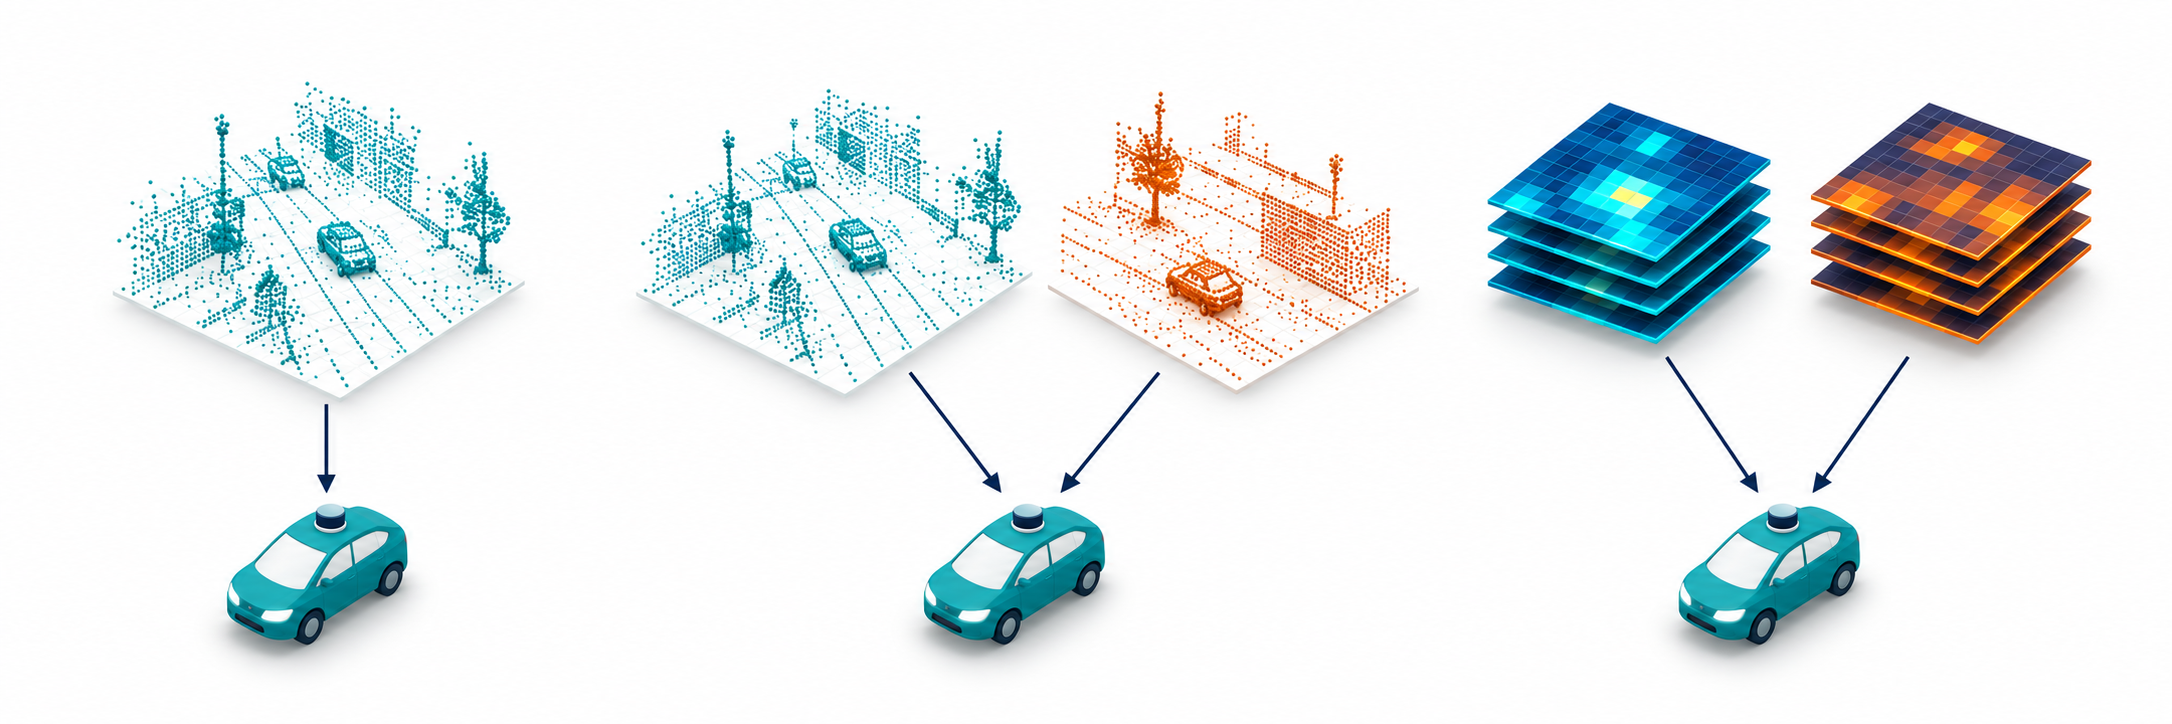
\includegraphics[width=12.0cm]{assets/illustrations/problem/problem-distillation-imagegen-v1.png}};
    \node[final statement,text width=14.4cm,
      font=\sffamily\fontsize{16}{20}\selectfont] at (7.4,5.28)
      {Can a Holistic Early-Fusion Model Be Compressed\\
      While Preserving Detection Accuracy?};
    \node[final heading] at (3.2,4.40) {Own Scan Only};
    \node[final heading] at (7.2,4.40) {Early Fusion};
    \node[final heading] at (11.3,4.40) {DiscoNet};
    \node[visual small,anchor=center] at (7.2,4.00) {Teacher};
    \node[visual small,anchor=center] at (11.3,4.00) {Student};
    \draw[visual arrow,dashed] (7.74,1.12) --
      node[above,align=center,text=MoverNavy,font=\fontsize{9}{11}\selectfont]
        {Distillation\\Training Only} (10.65,1.12);
    \node[final caption] at (3.2,0.34) {No Sharing};
    \node[final caption] at (7.2,0.34) {Holistic View};
    \node[final caption] at (11.3,0.34) {Learned Features};
  \end{VisualCanvas}}
  \SlideSource{Source: AI generated illustrations.}
\end{frame}
